\documentclass[useAMS,usenatbib,referee,12pt]{article}
\usepackage[margin=1.0in]{geometry}
\usepackage{placeins}     % Enables \FloatBarrier, which enforces a break between table/figures
\usepackage{multirow}     % Allows tables with vertically merged cells
\usepackage{xr}    % Links to external document
\usepackage{rotating}     % For landscape-oriented table

\graphicspath{{Sims/SimFull/}}

\externaldocument[M-]{Draft}

\newcommand{\pdet}{p^{(det)}}
\newcommand{\capt}[1]{Caterpillar plots of posterior parameter estimates from all models fit to the simulated #1 dataset (from simulations involving covariates and random effects).  Black and orange lines depict central 95\% and 50\% credible intervals, respectively.  The black dot is the posterior meadian.  The blue 'X' is the true parameter value and is positioned on the correctly specified model.  $\beta$'s are fixed effect parameters, $\sigma$'s are random effect standard deviations, and $\gamma$ is a mixing parameter.  Parameters designated with an 'A' are abundance parameters; those designated with a 'D' are detection parameters.}
\newcommand{\sfig}[2]{\begin{figure}
  \includegraphics[width=1.0\textwidth]{Posteriors_all_simdat#2.jpg} % Source file: Sims/SimFull/Outputs_Code_sf.R
  \caption{\capt{#1}}
  \end{figure}
}
\renewcommand{\thesection}{S-\arabic{section}}   % Label section with 'S-#'
\renewcommand{\thetable}{S-\arabic{table}}
\renewcommand{\thefigure}{S-\arabic{figure}}

\begin{document}

\section{Tables}
\begin{table}[!ht]
\centering
\begin{tabular}{lll|ccc}
  \hline
Family & Mixture & Peaked & $\gamma$ & $\varphi$ & $\alpha$ \\ 
  \hline
Exponential & Non-mixture & &  & -1.827 &  \\ 
  & Mixture & & 0.65 & -2.138 &  \\ 
  \hline
  Gamma & Non-mixture & Nonpeaked &  & -3.279 & 0.257 \\ 
  & & Peaked &  & -0.746 & 3.371 \\ 
  & Mixture & Nonpeaked & 0.65 & -2.773 & 0.577 \\ 
  & & Peaked & 0.65 & -1.210 & 2.491 \\ 
  \hline
  Lognormal & Non-mixture & Nonpeaked &  & -0.341 & 2.330 \\ 
  & & Peaked &  & -1.872 & 0.512 \\ 
  & Mixture & Nonpeaked & 0.65 & -1.462 & 1.674 \\ 
  & & Peaked & 0.65 & -1.992 & 0.618 \\ 
  \hline
  Weibull & Non-mixture & Nonpeaked &  & -1.165 & 0.418 \\ 
  & & Peaked &  & -2.042 & 1.829 \\ 
  & Mixture & Nonpeaked & 0.65 & -2.063 & 0.687 \\ 
  & & Peaked & 0.65 & -2.201 & 1.621 \\ 
   \hline
\end{tabular}
\caption{\label{simvals}Table of parameter values used to generate data for: (i) the mixture vs. non-mixture simulation, and (ii) the constant vs. non-constant rate simulation.  Here $\gamma$ is a mixing parameter for the proportion of `hard to detect' individuals, $\varphi$ is the detection rate parameter, and $\alpha$ is the shape parameter.}
\end{table}

\begin{sidewaystable}[h!]\footnotesize
\centering
\begin{tabular}{lll|rrrr|rrrrr}
  \hline
Family & Mixture & Peak & $\beta^A_1$ & $\beta^A_2$ & $\beta^A_3$ & $\beta^A_4$ & $\beta^D_1$ & $\beta^D_2$ & $\beta^D_3$ & $\beta^D_4$ & $\beta^D_5$  \\
  \hline
Exponential & Non-mixture & &0.122&0.002&0.094&-1.039&-0.01&-0.056&0.118&0.249&0.164 \\
& Mixture & &0.124&0.012&0.064&-1.07&-0.068&-0.146&0.03&0.312&0.27 \\
Gamma & Non-mixture & Nonpeaked &0.129&-0.001&0.098&-1.039&0.048&-0.104&-0.12&0.141&0.129 \\
& & Peaked &0.129&-0.001&0.098&-1.039&0.048&-0.104&-0.12&0.141&0.129 \\
& Mixture & Nonpeaked &0.128&-0.005&0.079&-1.051&-0.048&-0.126&-0.042&0.21&0.2 \\
& & Peaked &0.128&-0.005&0.079&-1.051&-0.048&-0.126&-0.042&0.21&0.2 \\
Lognormal & Non-mixture & Nonpeaked &0.126&0.031&0.096&-1.047&0.163&-0.099&-0.071&0.31&0.079 \\
& & Peaked &0.126&0.031&0.096&-1.047&0.163&-0.099&-0.071&0.31&0.079 \\
& Mixture & Nonpeaked &0.126&0.017&0.07&-1.068&0.006&-0.14&-0.038&0.341&0.191 \\
& & Peaked &0.126&0.017&0.07&-1.068&0.006&-0.14&-0.038&0.341&0.191 \\
Weibull & Non-mixture & Nonpeaked &0.129&0.011&0.102&-1.04&0.101&-0.104&-0.127&0.204&0.086 \\
& & Peaked &0.129&0.011&0.102&-1.04&0.101&-0.104&-0.127&0.204&0.086 \\
& Mixture & Nonpeaked &0.129&-0.002&0.081&-1.049&-0.028&-0.122&-0.069&0.204&0.183 \\
& & Peaked &0.129&-0.002&0.081&-1.049&-0.028&-0.122&-0.069&0.204&0.183 \\
  \hline
\end{tabular}\\
\vspace{1.25cm}
\begin{tabular}{ll|lrrrrrrr}
  \hline
Family & Mixture & Peak & Intercept$^A$ & Intercept$^D$ & $\sigma_{A1}$ & $\sigma_{A2}$ & $\sigma_D$ & $\gamma$ & $\alpha$ \\
\hline
Exponential & Non-mixture & &0.975&-1.146&0.139&0.094&0.242& & \\
& Mixture & &1.097&-1.97&0.13&0.091&0.259&0.647& \\
Gamma & Non-mixture & Nonpeaked &1.383&-3.941&0.121&0.072&0.39& & 0.316 \\
& & Peaked &1.134&-0.746&0.121&0.072&0.39& & 3.371 \\
& Mixture & Nonpeaked &1.215&-2.7&0.121&0.079&0.332&0.79& 0.597 \\
& & Peaked &1.134&-1.21&0.121&0.079&0.332&0.65& 2.491 \\
Lognormal & Non-mixture & Nonpeaked &1.613&-2.444&0.151&0.077&0.353& & 3.287 \\
& & Peaked &1.134&-1.872&0.151&0.077&0.353& & 0.512 \\
& Mixture & Nonpeaked &1.282&-2.051&0.14&0.079&0.312&0.706& 1.467 \\
& & Peaked &1.134&-1.992&0.14&0.079&0.312&0.65& 0.618 \\
Weibull & Non-mixture & Nonpeaked &1.57&-3.137&0.131&0.074&0.383& & 0.387 \\
& & Peaked &1.134&-2.042&0.131&0.074&0.383& & 1.829 \\
& Mixture & Nonpeaked &1.294&-2.354&0.122&0.078&0.344&0.814& 0.653 \\
& & Peaked &1.134&-2.201&0.122&0.078&0.344&0.65& 1.621 \\
   \hline
\end{tabular}
\caption{\label{tbl:sim3}Table of parameter values used to generate data for simulations with covariates (Section \ref{M-sec:simfull}).  Here, $\gamma$ is a mixing parameter for the proportion of `hard to detect' individuals, $\beta$'s are fixed effects, $\sigma$'s are random effect standard deviations, $\alpha$ is a shape parameter, and superscripts of $A$ and $D$ indicate abundance and detection parameters, respectively.}
\end{sidewaystable}


\begin{table}[ht]
\footnotesize\centering
\begin{tabular}{l|l|l|l|cccc|cccc}
 \multicolumn{4}{c|}{ } & \multicolumn{4}{c|}{\underline{Non-mixture model}} & \multicolumn{4}{c}{\underline{Mixture model}} \\
 \multicolumn{4}{c|}{ } & Med $p$ & Q($p$) & 50\% & 90\% & Med $p$ & Q($p$) & 50\% & 90\% \\ 
  \hline
  \hline
 \parbox[t]{2mm}{\multirow{14}{*}{\rotatebox[origin=c]{90}{TTDD used to simulate data}}} & \parbox[t]{2mm}{\multirow{7}{*}{\rotatebox[origin=c]{90}{Non-mixture}}} & \parbox[t]{2mm}{\multirow{3}{*}{\rotatebox[origin=c]{90}{Nonpk.}}} & Gamma & 0.67 & 0.84 & 0.11 & 0.94 & 0.76 & 0.92 & 0.00 & 0.70 \\ 
   &  &  & Lognormal & 0.54 & 0.60 & 0.81 & 1.00 & 0.68 & 0.88 & 0.05 & 0.79 \\ 
   &  &  & Weibull & 0.55 & 0.61 & 0.79 & 0.99 & 0.69 & 0.84 & 0.16 & 0.87 \\ 
  \cline{3-12}
 & & &  Exponential & 0.49 & 0.45 & 0.51 & 0.93 & 0.45 & 0.30 & 0.47 & 0.86 \\ 
  \cline{3-12}
 & & \parbox[t]{2mm}{\multirow{3}{*}{\rotatebox[origin=c]{90}{Peaked}}} & Gamma & 0.48 & 0.46 & 0.57 & 0.90 & 0.57 & 0.72 & 0.42 & 0.85 \\ 
   &  &  & Lognormal & 0.49 & 0.45 & 0.53 & 0.93 & 0.54 & 0.69 & 0.37 & 0.89 \\ 
   &  &  & Weibull & 0.48 & 0.48 & 0.40 & 0.91 & 0.59 & 0.74 & 0.37 & 0.80 \\ 
  \cline{2-12}
& \parbox[t]{2mm}{\multirow{7}{*}{\rotatebox[origin=c]{90}{Mixture}}} & \parbox[t]{2mm}{\multirow{3}{*}{\rotatebox[origin=c]{90}{Nonpk.}}} & Gamma & 0.62 & 0.76 & 0.42 & 0.99 & 0.71 & 0.86 & 0.10 & 0.89 \\ 
   &  &  & Lognormal & 0.50 & 0.47 & 0.95 & 1.00 & 0.64 & 0.84 & 0.09 & 0.97 \\ 
   &  &  & Weibull & 0.50 & 0.47 & 0.92 & 1.00 & 0.64 & 0.77 & 0.39 & 0.98 \\ 
  \cline{3-12}
 & & &   Exponential & 0.88 & 1.00 & 0.00 & 0.00 & 0.50 & 0.49 & 0.54 & 0.95 \\ 
  \cline{3-12}
 & & \parbox[t]{2mm}{\multirow{3}{*}{\rotatebox[origin=c]{90}{Peaked}}} & Gamma & 0.24 & 0.01 & 0.00 & 0.00 & 0.52 & 0.53 & 0.76 & 0.99 \\ 
   &  &  & Lognormal & 0.18 & 0.00 & 0.00 & 0.00 & 0.49 & 0.47 & 0.66 & 0.97 \\ 
   &  &  & Weibull & 0.18 & 0.00 & 0.00 & 0.00 & 0.52 & 0.52 & 0.80 & 1.00 \\ 
   \hline
\end{tabular}
\caption{Summary of mixture vs. non-mixture model fits when the detection probability is $\pdet =0.50$.  
In all cases, the inference model family matches the dataset family.  
Med $p$: average across simulations of the posterior median of $\pdet$.  
Q($p$): average proportion of the posterior distribution of $\pdet$ that is larger than the true value.  
50\% and 90\% coverage is expressed as the proportion of 100 simulations for which the true value of $\pdet$ lies within the appropriate credible interval.}
\label{tbl:mix50}

\vspace{1.2cm}

\begin{tabular}{l|l|l|l|cccc|cccc}
 \multicolumn{4}{c|}{ } & \multicolumn{4}{c|}{\underline{Non-mixture model}} & \multicolumn{4}{c}{\underline{Mixture model}} \\
 \multicolumn{4}{c|}{ } & Med $p$ & Q($p$) & 50\% & 90\% & Med $p$ & Q($p$) & 50\% & 90\% \\ 
  \hline
  \hline
 \parbox[t]{2mm}{\multirow{14}{*}{\rotatebox[origin=c]{90}{TTDD used to simulate data}}} & \parbox[t]{2mm}{\multirow{7}{*}{\rotatebox[origin=c]{90}{Non-mixture}}} & \parbox[t]{2mm}{\multirow{3}{*}{\rotatebox[origin=c]{90}{Nonpk.}}}& Gamma & 0.69 & 0.59 & 0.78 & 0.98 & 0.78 & 0.79 & 0.35 & 0.90 \\ 
   &  &  & Lognormal & 0.59 & 0.31 & 0.45 & 0.91 & 0.73 & 0.69 & 0.63 & 0.90 \\ 
   &  &  & Weibull & 0.60 & 0.38 & 0.59 & 0.99 & 0.73 & 0.68 & 0.59 & 0.94 \\
  \cline{3-12}
   &  &  & Exponential & 0.64 & 0.47 & 0.50 & 0.85 & 0.61 & 0.29 & 0.33 & 0.82 \\ 
  \cline{3-12}
 & & \parbox[t]{2mm}{\multirow{3}{*}{\rotatebox[origin=c]{90}{Peaked}}}& Gamma & 0.64 & 0.44 & 0.46 & 0.89 & 0.68 & 0.66 & 0.51 & 0.85 \\ 
   &  &  & Lognormal & 0.64 & 0.47 & 0.36 & 0.87 & 0.67 & 0.63 & 0.44 & 0.79 \\ 
   &  &  & Weibull & 0.61 & 0.40 & 0.46 & 0.88 & 0.69 & 0.67 & 0.46 & 0.88 \\ 
  \cline{2-12}
& \parbox[t]{2mm}{\multirow{7}{*}{\rotatebox[origin=c]{90}{Mixture}}} & \parbox[t]{2mm}{\multirow{3}{*}{\rotatebox[origin=c]{90}{Nonpk.}}}& Gamma & 0.60 & 0.36 & 0.78 & 1.00 & 0.71 & 0.63 & 0.81 & 0.99 \\ 
   &  &  & Lognormal & 0.52 & 0.13 & 0.12 & 0.74 & 0.67 & 0.54 & 0.93 & 1.00 \\ 
   &  &  & Weibull & 0.51 & 0.17 & 0.23 & 0.82 & 0.66 & 0.52 & 0.92 & 1.00 \\ 
  \cline{3-12}
   &  &  & Exponential & 0.93 & 1.00 & 0.00 & 0.00 & 0.63 & 0.46 & 0.45 & 0.87 \\ 
  \cline{3-12}
 & & \parbox[t]{2mm}{\multirow{3}{*}{\rotatebox[origin=c]{90}{Peaked}}} & Gamma & 0.26 & 0.00 & 0.00 & 0.00 & 0.58 & 0.34 & 0.51 & 0.95 \\ 
   &  &  & Lognormal & 0.20 & 0.00 & 0.00 & 0.00 & 0.61 & 0.41 & 0.58 & 0.92 \\ 
   &  &  & Weibull & 0.19 & 0.00 & 0.00 & 0.00 & 0.56 & 0.34 & 0.44 & 0.95 \\ 
   \hline
\end{tabular}
\caption{Summary of mixture vs. non-mixture model fits when the detection probability is $\pdet =0.65$.  
In all cases, the inference model family matches the dataset family.  
Med $p$: average across simulations of the posterior median of $\pdet$.  
Q($p$): average proportion of the posterior distribution of $\pdet$ that is larger than the true value.  
50\% and 90\% coverage is expressed as the proportion of 100 simulations for which the true value of $\pdet$ lies within the appropriate credible interval.}
\label{tbl:mix65}
\end{table}



\begin{table}[ht]\centering\footnotesize
\begin{tabular}{l|l|l|l|cccc|cccc}
 \multicolumn{4}{c|}{ } & \multicolumn{4}{c|}{\underline{Non-mixture model}} & \multicolumn{4}{c}{\underline{Mixture model}} \\
 \multicolumn{4}{c|}{ } & Med $p$ & Q($p$) & 50\% & 90\% & Med $p$ & Q($p$) & 50\% & 90\% \\ 
  \hline
  \hline
 \parbox[t]{2mm}{\multirow{14}{*}{\rotatebox[origin=c]{90}{TTDD used to simulate data}}} & \parbox[t]{2mm}{\multirow{7}{*}{\rotatebox[origin=c]{90}{Non-mixture}}} & \parbox[t]{2mm}{\multirow{3}{*}{\rotatebox[origin=c]{90}{Nonpk.}}} & Gamma & 0.75 & 0.39 & 0.45 & 0.92 & 0.83 & 0.62 & 0.55 & 0.91 \\ 
   &  &  & Lognormal & 0.71 & 0.29 & 0.29 & 0.82 & 0.82 & 0.61 & 0.63 & 0.91 \\ 
   &  &  & Weibull & 0.72 & 0.34 & 0.41 & 0.86 & 0.82 & 0.60 & 0.59 & 0.93 \\ 
  \cline{3-12}
    &  &  & Exponential & 0.80 & 0.49 & 0.54 & 0.88 & 0.78 & 0.32 & 0.48 & 0.86 \\ 
  \cline{3-12}
 & & \parbox[t]{2mm}{\multirow{3}{*}{\rotatebox[origin=c]{90}{Peaked}}} & Gamma & 0.79 & 0.44 & 0.45 & 0.87 & 0.81 & 0.59 & 0.45 & 0.90 \\ 
   &  &  & Lognormal & 0.80 & 0.48 & 0.52 & 0.95 & 0.81 & 0.60 & 0.53 & 0.92 \\ 
   &  &  & Weibull & 0.78 & 0.37 & 0.38 & 0.84 & 0.81 & 0.57 & 0.49 & 0.92 \\ 
  \cline{2-12}
& \parbox[t]{2mm}{\multirow{7}{*}{\rotatebox[origin=c]{90}{Mixture}}} & \parbox[t]{2mm}{\multirow{3}{*}{\rotatebox[origin=c]{90}{Nonpk.}}} & Gamma & 0.64 & 0.11 & 0.11 & 0.59 & 0.75 & 0.38 & 0.64 & 1.00 \\ 
   &  &  & Lognormal & 0.58 & 0.06 & 0.04 & 0.27 & 0.74 & 0.33 & 0.51 & 0.98 \\ 
   &  &  & Weibull & 0.54 & 0.04 & 0.01 & 0.23 & 0.70 & 0.27 & 0.46 & 1.00 \\ 
  \cline{3-12}
   &  &  & Exponential & 0.96 & 1.00 & 0.00 & 0.00 & 0.78 & 0.45 & 0.42 & 0.86 \\ 
  \cline{3-12}
 & & \parbox[t]{2mm}{\multirow{3}{*}{\rotatebox[origin=c]{90}{Peaked}}} & Gamma & 0.28 & 0.00 & 0.00 & 0.00 & 0.72 & 0.30 & 0.40 & 0.80 \\ 
   &  &  & Lognormal & 0.22 & 0.00 & 0.00 & 0.00 & 0.78 & 0.45 & 0.46 & 0.87 \\ 
   &  &  & Weibull & 0.22 & 0.00 & 0.00 & 0.00 & 0.69 & 0.29 & 0.33 & 0.88 \\ 
   \hline
\end{tabular}
\caption{Summary of mixture vs. non-mixture model fits when the detection probability is $\pdet =0.80$.  
In all cases, the inference model family matches the dataset family.  
Med $p$: average across simulations of the posterior median of $\pdet$.  
Q($p$): average proportion of the posterior distribution of $\pdet$ that is larger than the true value.  
50\% and 90\% coverage is expressed as the proportion of 100 simulations for which the true value of $\pdet$ lies within the appropriate credible interval.}
\label{tbl:mix80}

\vspace{1.2cm}

\begin{tabular}{l|l|l|l|cccc|cccc}
 \multicolumn{4}{c|}{ } & \multicolumn{4}{c|}{\underline{Non-mixture model}} & \multicolumn{4}{c}{\underline{Mixture model}} \\
 \multicolumn{4}{c|}{ } & Med $p$ & Q($p$) & 50\% & 90\% & Med $p$ & Q($p$) & 50\% & 90\% \\ 
  \hline
  \hline
 \parbox[t]{2mm}{\multirow{14}{*}{\rotatebox[origin=c]{90}{TTDD used to simulate data}}} & \parbox[t]{2mm}{\multirow{7}{*}{\rotatebox[origin=c]{90}{Non-mixture}}} & \parbox[t]{2mm}{\multirow{3}{*}{\rotatebox[origin=c]{90}{Nonpk.}}} & Gamma & 0.95 & 0.44 & 0.59 & 0.95 & 0.96 & 0.62 & 0.61 & 0.96 \\ 
   &  &  & Lognormal & 0.94 & 0.42 & 0.47 & 0.87 & 0.96 & 0.65 & 0.44 & 0.90 \\ 
   &  &  & Weibull & 0.94 & 0.46 & 0.43 & 0.90 & 0.96 & 0.67 & 0.52 & 0.84 \\ 
  \cline{3-12}
   &  &  & Exponential & 0.95 & 0.54 & 0.48 & 0.90 & 0.94 & 0.37 & 0.42 & 0.89 \\ 
  \cline{3-12}
 & & \parbox[t]{2mm}{\multirow{3}{*}{\rotatebox[origin=c]{90}{Peaked}}} & Gamma & 0.95 & 0.43 & 0.44 & 0.89 & 0.95 & 0.50 & 0.40 & 0.88 \\ 
   &  &  & Lognormal & 0.95 & 0.50 & 0.44 & 0.88 & 0.95 & 0.54 & 0.44 & 0.88 \\ 
   &  &  & Weibull & 0.95 & 0.53 & 0.49 & 0.91 & 0.96 & 0.65 & 0.42 & 0.85 \\ 
  \cline{2-12}
& \parbox[t]{2mm}{\multirow{7}{*}{\rotatebox[origin=c]{90}{Mixture}}} & \parbox[t]{2mm}{\multirow{3}{*}{\rotatebox[origin=c]{90}{Nonpk.}}} & Gamma & 0.85 & 0.04 & 0.03 & 0.22 & 0.91 & 0.25 & 0.31 & 0.77 \\ 
   &  &  & Lognormal & 0.85 & 0.03 & 0.03 & 0.16 & 0.92 & 0.28 & 0.38 & 0.86 \\ 
   &  &  & Weibull & 0.71 & 0.01 & 0.01 & 0.02 & 0.87 & 0.22 & 0.28 & 0.68 \\ 
  \cline{3-12}
   &  &  & Exponential & 0.99 & 1.00 & 0.00 & 0.00 & 0.94 & 0.41 & 0.51 & 0.85 \\ 
  \cline{3-12}
 & & \parbox[t]{2mm}{\multirow{3}{*}{\rotatebox[origin=c]{90}{Peaked}}} & Gamma & 0.37 & 0.00 & 0.00 & 0.00 & 0.94 & 0.39 & 0.41 & 0.83 \\ 
   &  &  & Lognormal & 0.27 & 0.00 & 0.00 & 0.00 & 0.94 & 0.40 & 0.43 & 0.83 \\ 
   &  &  & Weibull & 0.28 & 0.00 & 0.00 & 0.00 & 0.93 & 0.36 & 0.47 & 0.80 \\ 
   \hline
\end{tabular}
\caption{Summary of mixture vs. non-mixture model fits when the detection probability is $\pdet =0.95$.  
In all cases, the inference model family matches the dataset family.  
Med $p$: average across simulations of the posterior median of $\pdet$.  
Q($p$): average proportion of the posterior distribution of $\pdet$ that is larger than the true value.  
50\% and 90\% coverage is expressed as the proportion of 100 simulations for which the true value of $\pdet$ lies within the appropriate credible interval.}
\label{tbl:mix95}
\end{table}




\begin{table}[ht]\centering\footnotesize
\centering
\begin{tabular}{l|l|l|cccc|cccc}
 \multicolumn{3}{c}{ } & \multicolumn{4}{c}{\underline{Exponential mixture model}} & \multicolumn{4}{c}{\underline{Gamma mixture model}} \\
 \multicolumn{3}{c}{ } & Med $p$ & Q($p$) & 50\% & 90\%  & Med $p$ & Q($p$) & 50\% & 90\% \\ 
  \hline
\parbox[t]{2mm}{\multirow{7}{*}{\rotatebox[origin=c]{90}{Data Mixture}}} & \parbox[t]{2mm}{\multirow{3}{*}{\rotatebox[origin=c]{90}{Nonpk.}}} & Gamma & 0.84 & 0.99 & 0.00 & 0.05 & 0.71 & 0.86 & 0.10 & 0.89 \\ 
   &  & Lognormal & 0.89 & 1.00 & 0.00 & 0.00 & 0.78 & 0.93 & 0.01 & 0.56 \\ 
   &  & Weibull & 0.86 & 1.00 & 0.00 & 0.02 & 0.73 & 0.89 & 0.03 & 0.82 \\ 
\cline{2-11}
   &  & Exponential & 0.50 & 0.49 & 0.54 & 0.95 & 0.54 & 0.57 & 0.84 & 1.00 \\ 
\cline{2-11}
& \parbox[t]{2mm}{\multirow{3}{*}{\rotatebox[origin=c]{90}{Peaked}}} & Gamma & 0.31 & 0.06 & 0.05 & 0.32 & 0.52 & 0.53 & 0.76 & 0.99 \\ 
   &  & Lognormal & 0.26 & 0.02 & 0.00 & 0.09 & 0.59 & 0.68 & 0.52 & 0.91 \\ 
   &  & Weibull & 0.30 & 0.05 & 0.05 & 0.28 & 0.49 & 0.46 & 0.75 & 1.00 \\ 
   \hline
\end{tabular}
\vspace{0.5cm}\\
\begin{tabular}{l|l|l|cccc|cccc}
 \multicolumn{3}{c}{ } & \multicolumn{4}{c}{\underline{Lognormal mixture model}} & \multicolumn{4}{c}{\underline{Weibull mixture model}} \\
 \multicolumn{3}{c}{ } & Med $p$ & Q($p$) & 50\% & 90\% & Med $p$ & Q($p$) & 50\% & 90\% \\ 
  \hline
\parbox[t]{2mm}{\multirow{7}{*}{\rotatebox[origin=c]{90}{Data Mixture}}} & \parbox[t]{2mm}{\multirow{3}{*}{\rotatebox[origin=c]{90}{Nonpk.}}} & Gamma & 0.63 & 0.80 & 0.23 & 0.99 & 0.63 & 0.74 & 0.54 & 0.98 \\ 
   &  & Lognormal & 0.64 & 0.84 & 0.09 & 0.97 & 0.68 & 0.83 & 0.21 & 0.95 \\ 
   &  & Weibull & 0.63 & 0.81 & 0.18 & 0.99 & 0.64 & 0.77 & 0.39 & 0.98 \\ 
\cline{2-11}
   &  & Exponential & 0.49 & 0.45 & 0.77 & 1.00 & 0.54 & 0.56 & 0.87 & 0.99 \\ 
\cline{2-11}
& \parbox[t]{2mm}{\multirow{3}{*}{\rotatebox[origin=c]{90}{Peaked}}} & Gamma & 0.45 & 0.36 & 0.60 & 1.00 & 0.55 & 0.58 & 0.77 & 0.98 \\ 
   &  & Lognormal & 0.49 & 0.47 & 0.66 & 0.97 & 0.64 & 0.75 & 0.43 & 0.87 \\ 
   &  & Weibull & 0.43 & 0.30 & 0.51 & 0.97 & 0.52 & 0.52 & 0.80 & 1.00 \\ 
   \hline
\end{tabular}
\caption{Summary of models fits across family of TTDD when true detection probability is $\pdet = 0.50$.
All data and inference models have mixture components.
Med $p$: average across simulations of the posterior median of $\pdet$.  
Q($p$): average proportion of the posterior distribution of $\pdet$ that is larger than the true value.  
50\% and 90\% coverage is expressed as the proportion of simulations for which the true value of $\pdet$ lies within the appropriate credible interval.}
\label{tbl:fam50}

\vspace{0.5cm}
% Note: both tables are in the same 'table' environment.

\begin{tabular}{l|l|l|cccc|cccc}
 \multicolumn{3}{c}{ } & \multicolumn{4}{c}{\underline{Exponential mixture model}} & \multicolumn{4}{c}{\underline{Gamma mixture model}} \\
 \multicolumn{3}{c}{ } & Med $p$ & Q($p$) & 50\% & 90\%  & Med $p$ & Q($p$) & 50\% & 90\% \\ 
  \hline
\parbox[t]{2mm}{\multirow{7}{*}{\rotatebox[origin=c]{90}{Data Mixture}}} & \parbox[t]{2mm}{\multirow{3}{*}{\rotatebox[origin=c]{90}{Nonpk.}}} & Gamma & 0.83 & 0.96 & 0.04 & 0.21 & 0.71 & 0.63 & 0.81 & 0.99 \\ 
   &  & Lognormal & 0.91 & 1.00 & 0.00 & 0.00 & 0.82 & 0.86 & 0.19 & 0.70 \\ 
   &  & Weibull & 0.87 & 0.98 & 0.01 & 0.09 & 0.75 & 0.72 & 0.54 & 0.97 \\ 
\cline{2-11}
   &  & Exponential & 0.63 & 0.46 & 0.45 & 0.87 & 0.60 & 0.38 & 0.70 & 1.00 \\ 
\cline{2-11}
& \parbox[t]{2mm}{\multirow{3}{*}{\rotatebox[origin=c]{90}{Peaked}}} & Gamma & 0.33 & 0.01 & 0.02 & 0.05 & 0.58 & 0.34 & 0.51 & 0.95 \\ 
   &  & Lognormal & 0.30 & 0.00 & 0.00 & 0.00 & 0.71 & 0.68 & 0.48 & 0.88 \\ 
   &  & Weibull & 0.32 & 0.00 & 0.00 & 0.00 & 0.53 & 0.25 & 0.31 & 0.89 \\ 
   \hline
\end{tabular}
\vspace{0.5cm}\\
\begin{tabular}{l|l|l|cccc|cccc}
 \multicolumn{3}{c}{ } & \multicolumn{4}{c}{\underline{Lognormal mixture model}} & \multicolumn{4}{c}{\underline{Weibull mixture model}} \\
 \multicolumn{3}{c}{ } & Med $p$ & Q($p$) & 50\% & 90\% & Med $p$ & Q($p$) & 50\% & 90\% \\ 
  \hline
\parbox[t]{2mm}{\multirow{7}{*}{\rotatebox[origin=c]{90}{Data Mixture}}} & \parbox[t]{2mm}{\multirow{3}{*}{\rotatebox[origin=c]{90}{Nonpk.}}} & Gamma & 0.63 & 0.43 & 0.87 & 1.00 & 0.63 & 0.45 & 0.94 & 1.00 \\ 
   &  & Lognormal & 0.67 & 0.54 & 0.93 & 1.00 & 0.73 & 0.66 & 0.68 & 0.98 \\ 
   &  & Weibull & 0.64 & 0.46 & 0.97 & 1.00 & 0.66 & 0.52 & 0.92 & 1.00 \\ 
\cline{2-11}
   &  & Exponential & 0.55 & 0.24 & 0.39 & 0.95 & 0.58 & 0.36 & 0.69 & 1.00 \\ 
\cline{2-11}
& \parbox[t]{2mm}{\multirow{3}{*}{\rotatebox[origin=c]{90}{Peaked}}} & Gamma & 0.50 & 0.16 & 0.21 & 0.65 & 0.62 & 0.44 & 0.59 & 0.98 \\ 
   &  & Lognormal & 0.61 & 0.41 & 0.58 & 0.92 & 0.77 & 0.79 & 0.34 & 0.78 \\ 
   &  & Weibull & 0.47 & 0.11 & 0.13 & 0.48 & 0.56 & 0.34 & 0.44 & 0.95 \\ 
   \hline
\end{tabular}
\caption{Summary of models fits across family of TTDD when true detection probability is $\pdet = 0.65$.
All data and inference models have mixture components.
Med $p$: average across simulations of the posterior median of $\pdet$.  
Q($p$): average proportion of the posterior distribution of $\pdet$ that is larger than the true value.  
50\% and 90\% coverage is expressed as the proportion of simulations for which the true value of $\pdet$ lies within the appropriate credible interval.}
\label{tbl:fam65}
\end{table}




\begin{table}[ht]
\footnotesize\centering
\begin{tabular}{l|l|l|cccc|cccc}
 \multicolumn{3}{c}{ } & \multicolumn{4}{c}{\underline{Exponential mixture model}} & \multicolumn{4}{c}{\underline{Gamma mixture model}} \\
 \multicolumn{3}{c}{ } & Med $p$ & Q($p$) & 50\% & 90\%  & Med $p$ & Q($p$) & 50\% & 90\% \\ 
  \hline
\parbox[t]{2mm}{\multirow{7}{*}{\rotatebox[origin=c]{90}{Data Mixture}}} & \parbox[t]{2mm}{\multirow{3}{*}{\rotatebox[origin=c]{90}{Nonpk.}}} & Gamma & 0.86 & 0.83 & 0.25 & 0.59 & 0.75 & 0.38 & 0.64 & 1.00 \\ 
   &  & Lognormal & 0.93 & 1.00 & 0.00 & 0.01 & 0.88 & 0.80 & 0.33 & 0.72 \\ 
   &  & Weibull & 0.89 & 0.93 & 0.11 & 0.36 & 0.79 & 0.49 & 0.66 & 0.99 \\ 
\cline{2-11}
   &  & Exponential & 0.78 & 0.45 & 0.42 & 0.86 & 0.70 & 0.25 & 0.32 & 0.91 \\ 
\cline{2-11}
& \parbox[t]{2mm}{\multirow{3}{*}{\rotatebox[origin=c]{90}{Peaked}}} & Gamma & 0.37 & 0.00 & 0.00 & 0.00 & 0.72 & 0.30 & 0.40 & 0.80 \\ 
   &  & Lognormal & 0.34 & 0.00 & 0.00 & 0.00 & 0.85 & 0.77 & 0.24 & 0.65 \\ 
   &  & Weibull & 0.38 & 0.00 & 0.00 & 0.00 & 0.65 & 0.16 & 0.22 & 0.54 \\ 
   \hline
\end{tabular}
\vspace{0.5cm}\\
\begin{tabular}{l|l|l|cccc|cccc}
 \multicolumn{3}{c}{ } & \multicolumn{4}{c}{\underline{Lognormal mixture model}} & \multicolumn{4}{c}{\underline{Weibull mixture model}} \\
 \multicolumn{3}{c}{ } & Med $p$ & Q($p$) & 50\% & 90\% & Med $p$ & Q($p$) & 50\% & 90\% \\ 
  \hline
\parbox[t]{2mm}{\multirow{7}{*}{\rotatebox[origin=c]{90}{Data Mixture}}} & \parbox[t]{2mm}{\multirow{3}{*}{\rotatebox[origin=c]{90}{Nonpk.}}} & Gamma & 0.65 & 0.16 & 0.16 & 0.85 & 0.67 & 0.23 & 0.34 & 0.99 \\ 
   &  & Lognormal & 0.74 & 0.33 & 0.51 & 0.98 & 0.81 & 0.55 & 0.59 & 0.97 \\ 
   &  & Weibull & 0.66 & 0.17 & 0.22 & 0.87 & 0.70 & 0.27 & 0.46 & 1.00 \\ 
\cline{2-11}
   &  & Exponential & 0.61 & 0.11 & 0.12 & 0.52 & 0.64 & 0.21 & 0.24 & 0.85 \\ 
\cline{2-11}
& \parbox[t]{2mm}{\multirow{3}{*}{\rotatebox[origin=c]{90}{Peaked}}} & Gamma & 0.64 & 0.09 & 0.10 & 0.41 & 0.77 & 0.49 & 0.46 & 0.93 \\ 
   &  & Lognormal & 0.78 & 0.45 & 0.46 & 0.87 & 0.90 & 0.90 & 0.13 & 0.40 \\ 
   &  & Weibull & 0.57 & 0.04 & 0.02 & 0.19 & 0.69 & 0.29 & 0.33 & 0.88 \\ 
   \hline
\end{tabular}
\caption{Summary of models fits across family of TTDD when true detection probability is $\pdet = 0.80$.
All data and inference models have mixture components.
Med $p$: average across simulations of the posterior median of $\pdet$.  
Q($p$): average proportion of the posterior distribution of $\pdet$ that is larger than the true value.  
50\% and 90\% coverage is expressed as the proportion of simulations for which the true value of $\pdet$ lies within the appropriate credible interval.}
\label{tbl:fam80}

\vspace{0.5cm}

\begin{tabular}{l|l|l|cccc|cccc}
 \multicolumn{3}{c}{ } & \multicolumn{4}{c}{\underline{Exponential mixture model}} & \multicolumn{4}{c}{\underline{Gamma mixture model}} \\
 \multicolumn{3}{c}{ } & Med $p$ & Q($p$) & 50\% & 90\%  & Med $p$ & Q($p$) & 50\% & 90\% \\ 
  \hline
\parbox[t]{2mm}{\multirow{7}{*}{\rotatebox[origin=c]{90}{Data Mixture}}} & \parbox[t]{2mm}{\multirow{3}{*}{\rotatebox[origin=c]{90}{Nonpk.}}} & Gamma & 0.94 & 0.30 & 0.38 & 0.83 & 0.91 & 0.25 & 0.31 & 0.77 \\ 
   &  & Lognormal & 0.97 & 0.91 & 0.07 & 0.44 & 0.96 & 0.72 & 0.46 & 0.82 \\ 
   &  & Weibull & 0.94 & 0.29 & 0.37 & 0.76 & 0.91 & 0.25 & 0.32 & 0.76 \\ 
\cline{2-11}
   &  & Exponential & 0.94 & 0.41 & 0.51 & 0.85 & 0.92 & 0.26 & 0.33 & 0.82 \\ 
\cline{2-11}
& \parbox[t]{2mm}{\multirow{3}{*}{\rotatebox[origin=c]{90}{Peaked}}} & Gamma & 0.55 & 0.00 & 0.00 & 0.00 & 0.94 & 0.39 & 0.41 & 0.83 \\ 
   &  & Lognormal & 0.47 & 0.00 & 0.00 & 0.00 & 0.97 & 0.80 & 0.27 & 0.65 \\ 
   &  & Weibull & 0.57 & 0.00 & 0.00 & 0.00 & 0.89 & 0.08 & 0.09 & 0.43 \\ 
   \hline
\end{tabular}
\vspace{0.5cm}\\
\begin{tabular}{l|l|l|cccc|cccc}
 \multicolumn{3}{c}{ } & \multicolumn{4}{c}{\underline{Lognormal mixture model}} & \multicolumn{4}{c}{\underline{Weibull mixture model}} \\
 \multicolumn{3}{c}{ } & Med $p$ & Q($p$) & 50\% & 90\% & Med $p$ & Q($p$) & 50\% & 90\% \\ 
  \hline
\parbox[t]{2mm}{\multirow{7}{*}{\rotatebox[origin=c]{90}{Data Mixture}}} & \parbox[t]{2mm}{\multirow{3}{*}{\rotatebox[origin=c]{90}{Nonpk.}}} & Gamma & 0.81 & 0.11 & 0.10 & 0.35 & 0.87 & 0.23 & 0.22 & 0.68 \\ 
   &  & Lognormal & 0.92 & 0.28 & 0.38 & 0.86 & 0.95 & 0.55 & 0.57 & 0.92 \\ 
   &  & Weibull & 0.82 & 0.10 & 0.15 & 0.34 & 0.87 & 0.22 & 0.28 & 0.68 \\ 
\cline{2-11}
   &  & Exponential & 0.82 & 0.09 & 0.09 & 0.38 & 0.88 & 0.20 & 0.25 & 0.65 \\ 
\cline{2-11}
& \parbox[t]{2mm}{\multirow{3}{*}{\rotatebox[origin=c]{90}{Peaked}}}  & Gamma & 0.91 & 0.09 & 0.10 & 0.42 & 0.97 & 0.79 & 0.26 & 0.63 \\ 
   &  & Lognormal & 0.94 & 0.40 & 0.43 & 0.83 & 0.98 & 0.98 & 0.01 & 0.12 \\ 
   &  & Weibull & 0.84 & 0.01 & 0.00 & 0.03 & 0.93 & 0.36 & 0.47 & 0.80 \\ 
   \hline
\end{tabular}
\caption{Summary of models fits across family of TTDD when true detection probability is $\pdet = 0.95$.
All data and inference models have mixture components.
Med $p$: average across simulations of the posterior median of $\pdet$.  
Q($p$): average proportion of the posterior distribution of $\pdet$ that is larger than the true value.  
50\% and 90\% coverage is expressed as the proportion of simulations for which the true value of $\pdet$ lies within the appropriate credible interval.}
\label{tbl:fam95}
\end{table}

\FloatBarrier



\section{Figures}

\begin{figure}[h!]\centering
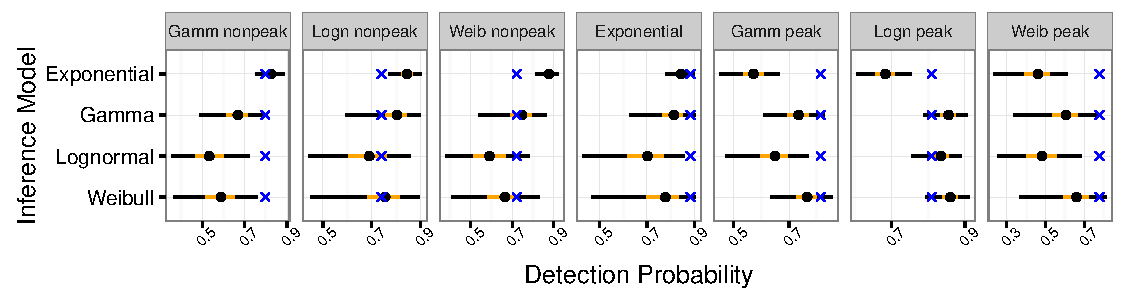
\includegraphics[width=0.98\textwidth]{pdet_cater_family} % Source file: Sims/SimFull/Outputs_Code_sf.R
\caption{\label{pdet_cater_family}  Simulation results from Section \ref{M-sec:simfull}.
Caterpillar plots of posterior 50\% (orange) and 95\% (black) credible intervals for the probability of detection $\pdet$ across all surveys.
Data and models include fixed and random effects for both abundance and detection processes.
All data and inference models include mixture components.  
Each plot presents one simulated dataset.  
`X' marks the expected marginal probability of detection based on true parameter values.}
\end{figure}


\subsection{Posterior parameter estimates from simulations including covariates and random effects}\label{s:sim3}
\sfig{non-mixture exponential}{1}
\sfig{exponential mixture}{2}
\sfig{nonpeaked non-mixture gamma}{3}
\sfig{nonpeaked gamma mixture}{4}
\sfig{peaked non-mixture gamma}{5}
\sfig{peaked gamma mixture}{6}
\sfig{nonpeaked non-mixture lognormal}{7}
\sfig{nonpeaked lognormal mixture}{8}
\sfig{peaked non-mixture lognormal}{9}
\sfig{peaked lognormal mixture}{10}
\sfig{nonpeaked non-mixture Weibull}{11}
\sfig{nonpeaked Weibull mixture}{12}
\sfig{peaked non-mixture Weibull}{13}
\sfig{peaked Weibull mixture}{14}

\end{document}
